\documentclass[10pt,a4paper]{article}
\usepackage[utf8]{inputenc}

% \usepackage{ngerman}  % german documents
\usepackage{graphicx}  % import graphics einbinden
\usepackage{listings}  % support source code listing
\usepackage{amsmath}  % math stuff
\usepackage{amssymb} % 
\usepackage{a4wide} % wide pages
\usepackage{fancyhdr} % nice headers
\usepackage{float}
\usepackage{longtable}
\usepackage{xcolor}
\usepackage{booktabs}
\definecolor{darkpastelgreen}{rgb}{0.01, 0.75, 0.24}
\definecolor{spirodiscoball}{rgb}{0.06, 0.75, 0.99}
\definecolor{smalt}{rgb}{0.0, 0.2, 0.6}
\definecolor{armygreen}{rgb}{0.29, 0.33, 0.13}
\definecolor{awesome}{rgb}{1.0, 0.13, 0.32}
\definecolor{bittersweet}{rgb}{1.0, 0.44, 0.37}
\definecolor{bananayellow}{rgb}{1.0, 0.88, 0.21}
\definecolor{blue}{rgb}{0.0, 0.0, 1.0}
\definecolor{red}{rgb}{1.0, 0.0, 0.0}
\definecolor{green}{rgb}{0.0, 1.0, 0.0}

% for multiple figures
\usepackage{subcaption}


\lstset{basicstyle=\footnotesize,language=Python,breaklines=true,numbers=left, numberstyle=\tiny, stepnumber=5,firstnumber=0, numbersep=5pt} % set up listings
\pagestyle{fancy}             % header
\setlength{\parindent}{0pt}   % no indentation
 

\usepackage[pdfpagemode=None, colorlinks=true,  % url coloring
           linkcolor=blue, urlcolor=blue, citecolor=blue, plainpages=false, 
           pdfpagelabels,unicode]{hyperref}
           
% change enums style: first level (a), (b), (c)           
\renewcommand{\labelenumi}{(\alph{enumi})}
\renewcommand{\labelenumii}{(\arabic{enumii})}

\newcommand{\norm}[1]{\left\lVert#1\right\rVert}

%lecture name
\newcommand{\lecture}{
	Bioinformatics III
}           

%assignment iteration
\newcommand{\assignment}{
	Eighth Assignment
}


%set up names, matricle number, and email
\newcommand{\authors}{
  \begin{tabular}{rl}
    \href{mailto:s8tbscho@stud.uni-saarland.de}{Thibault Schowing} & (2571837)\\
    \href{mailto:wiebkeschmitt@outlook.de}{Wiebke Schmitt} & (2543675)
  \end{tabular}
}

% use to start a new exercise
\newcommand{\exercise}[1]
{
  \stepcounter{subsection}
  \subsection*{Exercise \thesubsection: #1}

}

\begin{document}
\title{\Large \lecture \\ \textbf{\normalsize \assignment}}
\author{\authors}

\setlength \headheight{25pt}
\fancyhead[R]{\begin{tabular}{r}\lecture \\ \assignment \end{tabular}}
\fancyhead[L]{\authors}


\setcounter{section}{8} % modify for later sheets, i.e. 2, 3, ...
%\section{Introduction to Python and some Network Properties} % optional, note that section invocation sets the section counter + 1, so adapt the setcounter command
\maketitle

%EXERCICE 1
\exercise{Data Preprocessing}

\begin{enumerate}

% A
\item \textbf{Data matrix:}\textit{The supplement contains the data\string_matrix.py–file with the outline of a
	DataMatrix–class in which you should complete. }\\ 

\lstinputlisting[label=qtew-1, caption={Data Matrix class script}] {../Scripts/data\string_matrix.py}


%B
\item \textbf{Process expression and methylation data:}\textit{In the function exercise 1() in main.py,
	use your DataMatrix–class to read in the expression and methylation tables given in the
	supplement and write the processed matrices into files.} \footnote{The files are attached with the source files in the email.}\\

\lstinputlisting[label=qtew-1, caption={Main programm}] {../Scripts/main.py}


\textit{For each input file, report the number of genes and samples whose data does not follow a
	normal distribution with $\alpha$ = 0.05.
}\\

Number of genes whose data does not follow a normal distribution (EXPRESSION):  73\\

Number of sample whose data does not follow a normal distribution (EXPRESSION):  19\\

Number of genes whose data does not follow a normal distribution (METHYLATION):  66\\

Number of sample whose data does not follow a normal distribution (METHYLATION):  19\\



\end{enumerate}


%\newpage
%\lstinputlisting[label=qtew-1, caption={boolean\textunderscore network.py}] {../Scripts/boolean\string_network.py}
%\newpage
%\lstinputlisting[label=qtew-1, caption={Main function that tests the boolean network}] {../Scripts/main\string_boolean.py}




% NEW EXERCICE
\newpage
\exercise{Correlation Measures}
\lstinputlisting[label=qtew-1, caption={Correlation matrix}] {../Scripts/correlation.py}



% NEW EXERCICE
\newpage
\exercise{Gene Co–Expression Networks}
\begin{enumerate}
	
	% A
	\item \textbf{Network construction}\\
	
	\lstinputlisting[label=lsdddt-1, caption={Correlation network}] {../Scripts/network.py}
	
	
	% B
	\item \textbf{Network visualisation\footnote{The files are attached with the source files in the email.}}
	
	
\begin{figure}[H]
	\centering
	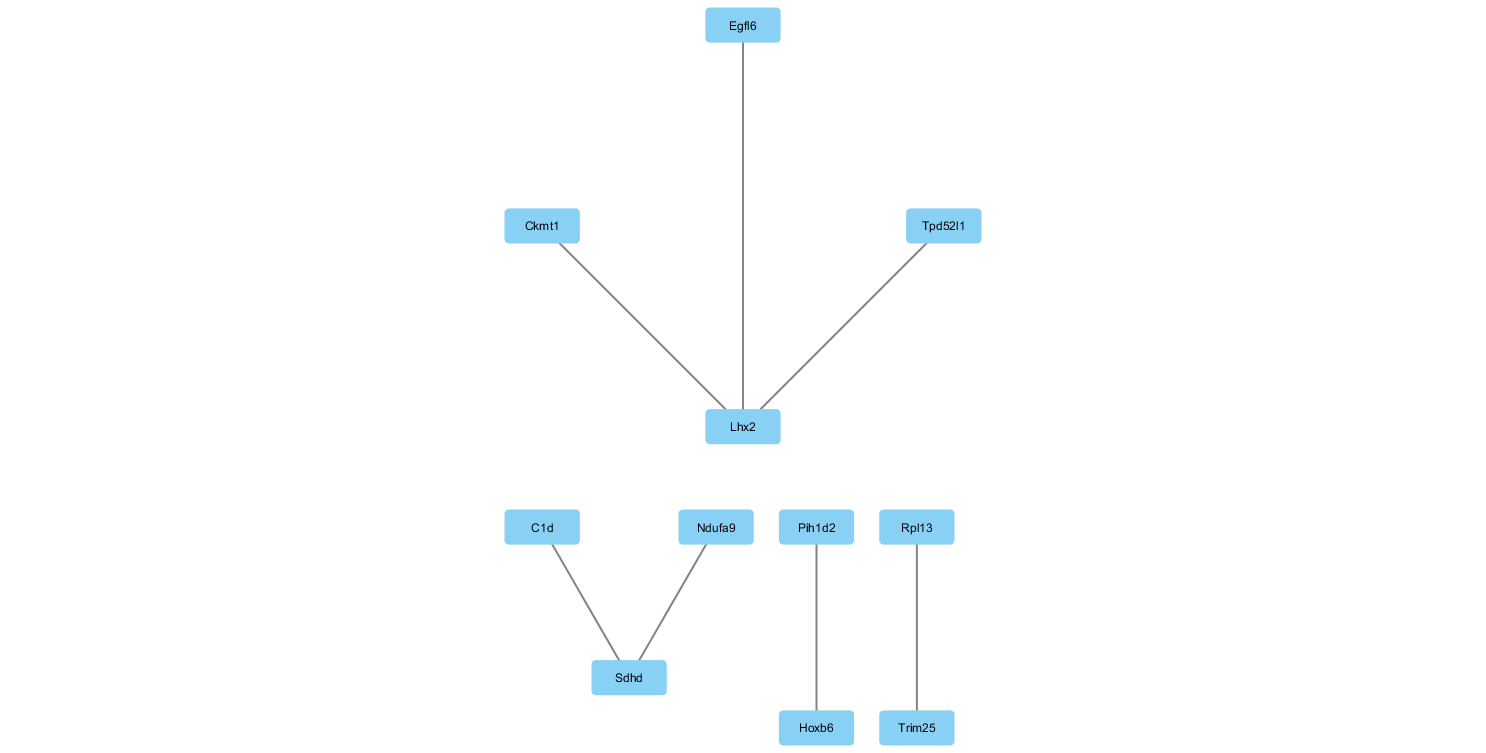
\includegraphics[width=0.9\linewidth]{img/schmitt_schowing_expression_network_kendall.png}
	\caption{Expression network with Kendall correlation}
	\label{fig:schmittschowingexpressionnetworkkendall}
\end{figure}

	
\begin{figure}[H]
	\centering
	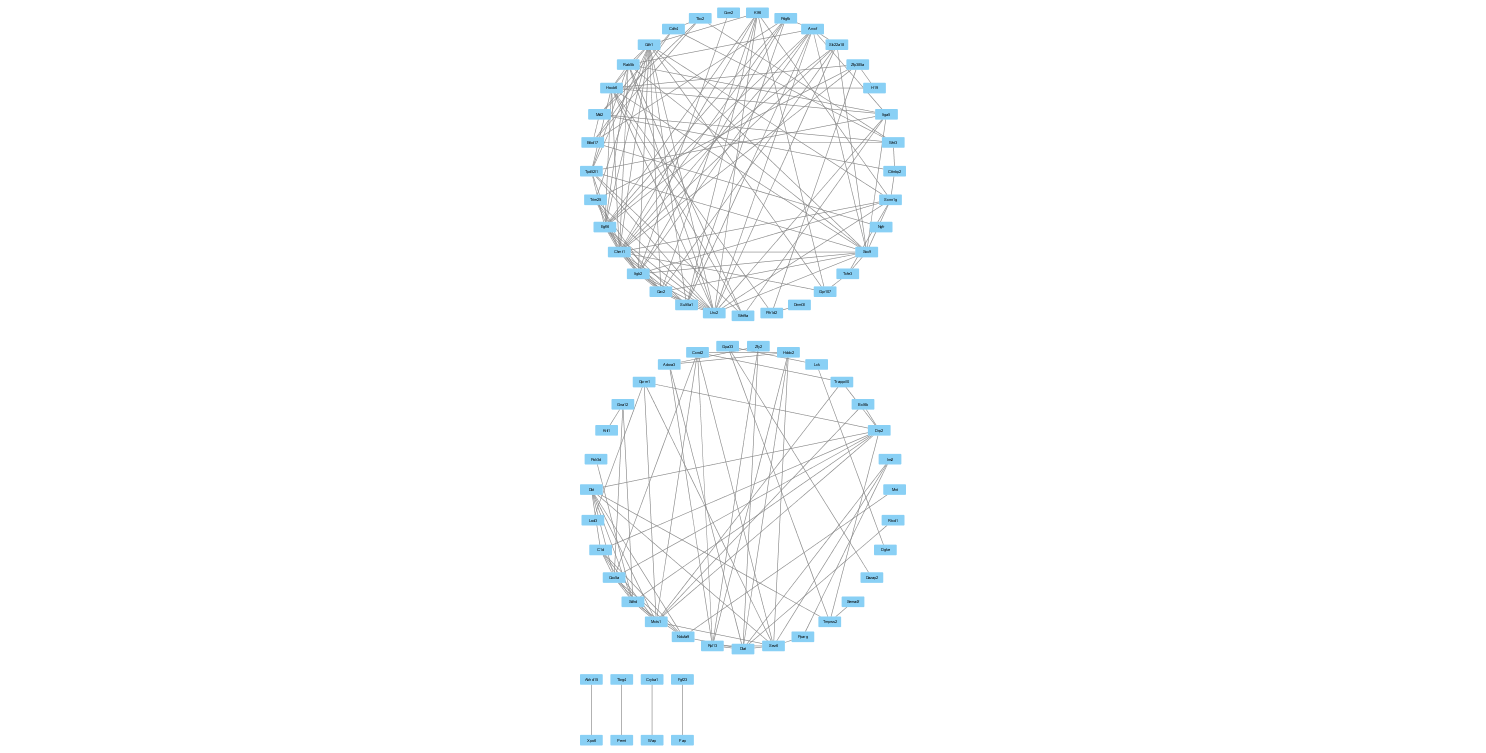
\includegraphics[width=0.9\linewidth]{img/schmitt_schowing_expression_network_pearson.png}
	\caption{Expression network with Pearson correlation}
	\label{fig:schmittschowingexpressionnetworkpearson}
\end{figure}

	
\begin{figure}[H]
	\centering
	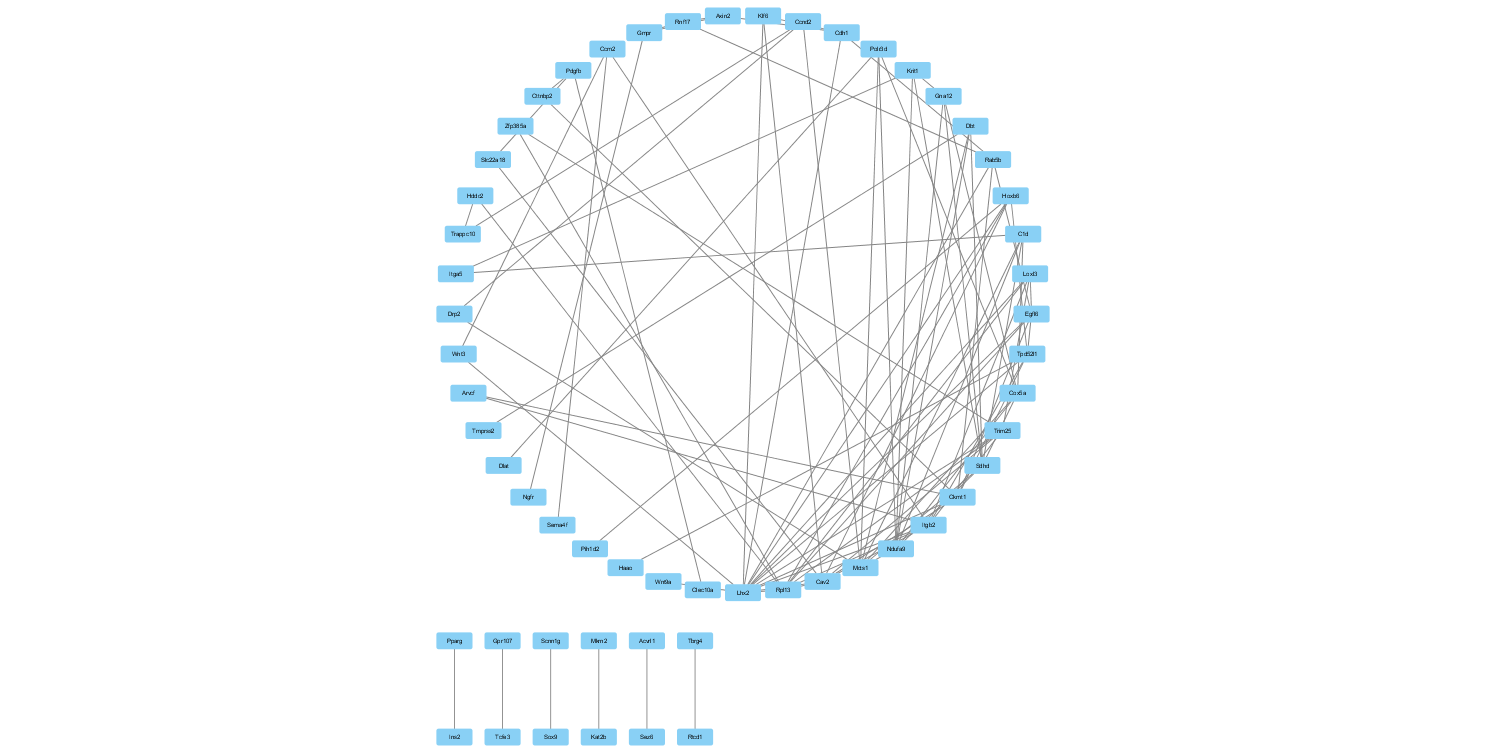
\includegraphics[width=0.9\linewidth]{img/schmitt_schowing_expression_network_spearman.png}
	\caption{Expression network with Spearman correlation}
	\label{fig:schmittschowingexpressionnetworkspearman}
\end{figure}


\begin{figure}[H]
	\centering
	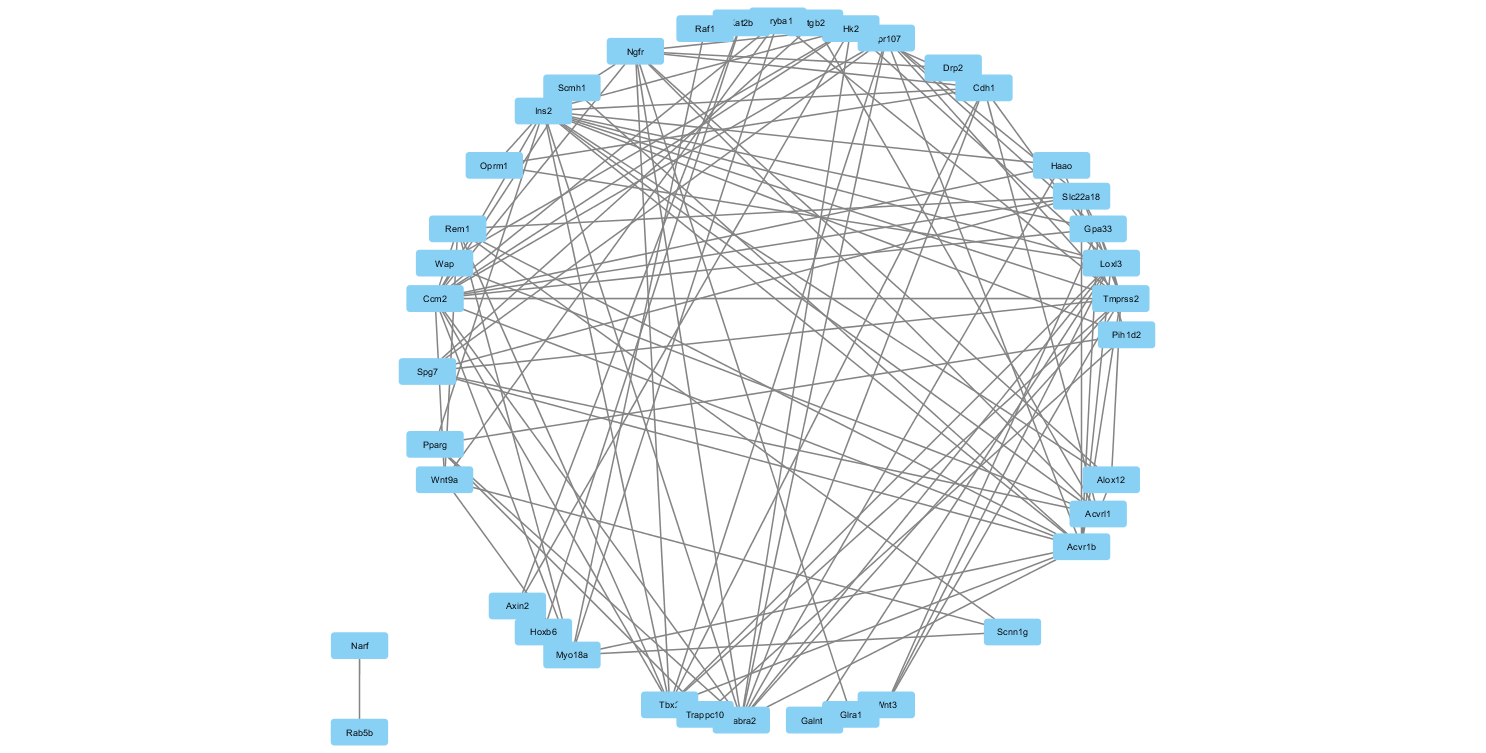
\includegraphics[width=0.9\linewidth]{img/schmitt_schowing_methylation_network_kendall}
	\caption{Methylation network with Kendall correlation}
	\label{fig:schmittschowingmethylationnetworkkendall}
\end{figure}



\begin{figure}[H]
	\centering
	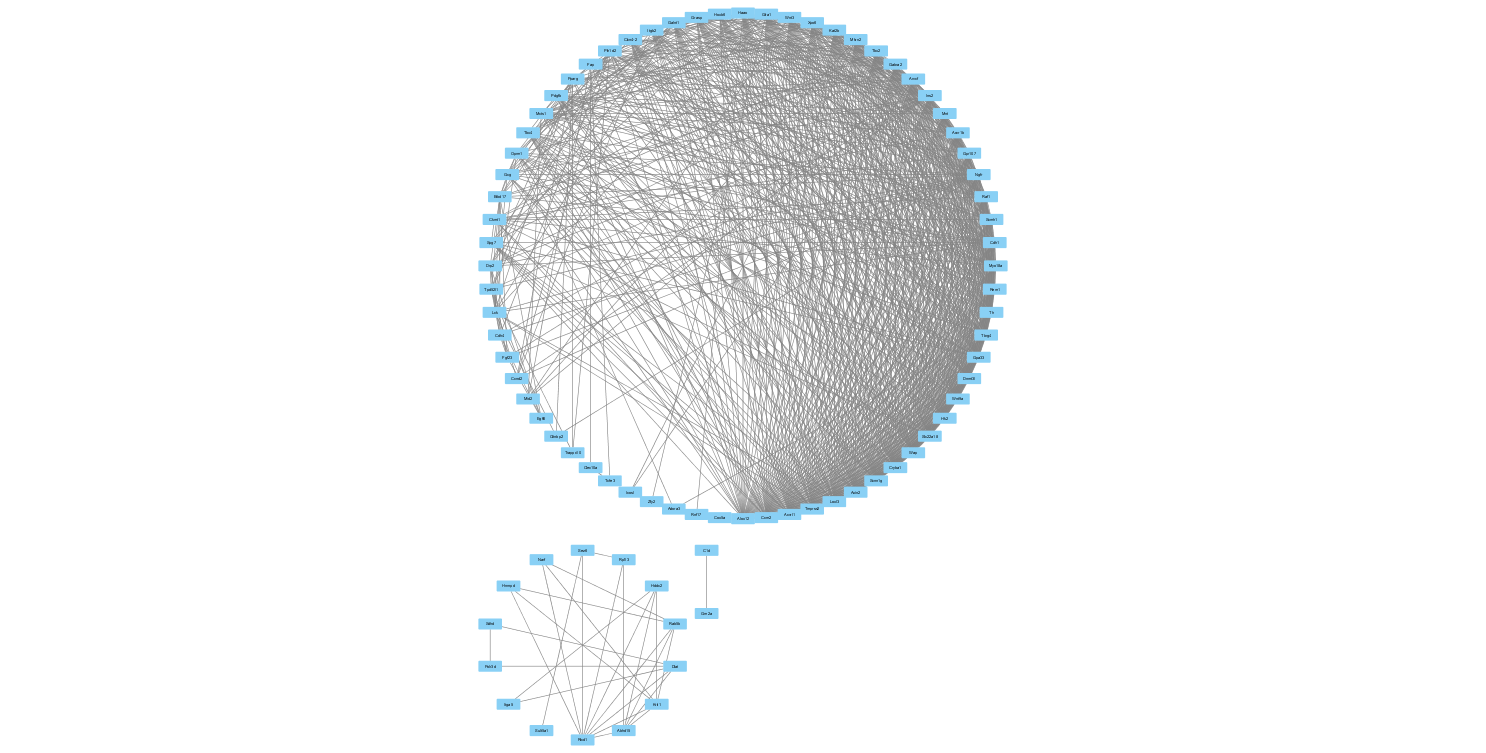
\includegraphics[width=0.9\linewidth]{img/schmitt_schowing_methylation_network_pearson}
	\caption{Methylation network with Pearson correlation}
	\label{fig:schmittschowingmethylationnetworkpearson}
\end{figure}


\begin{figure}[H]
	\centering
	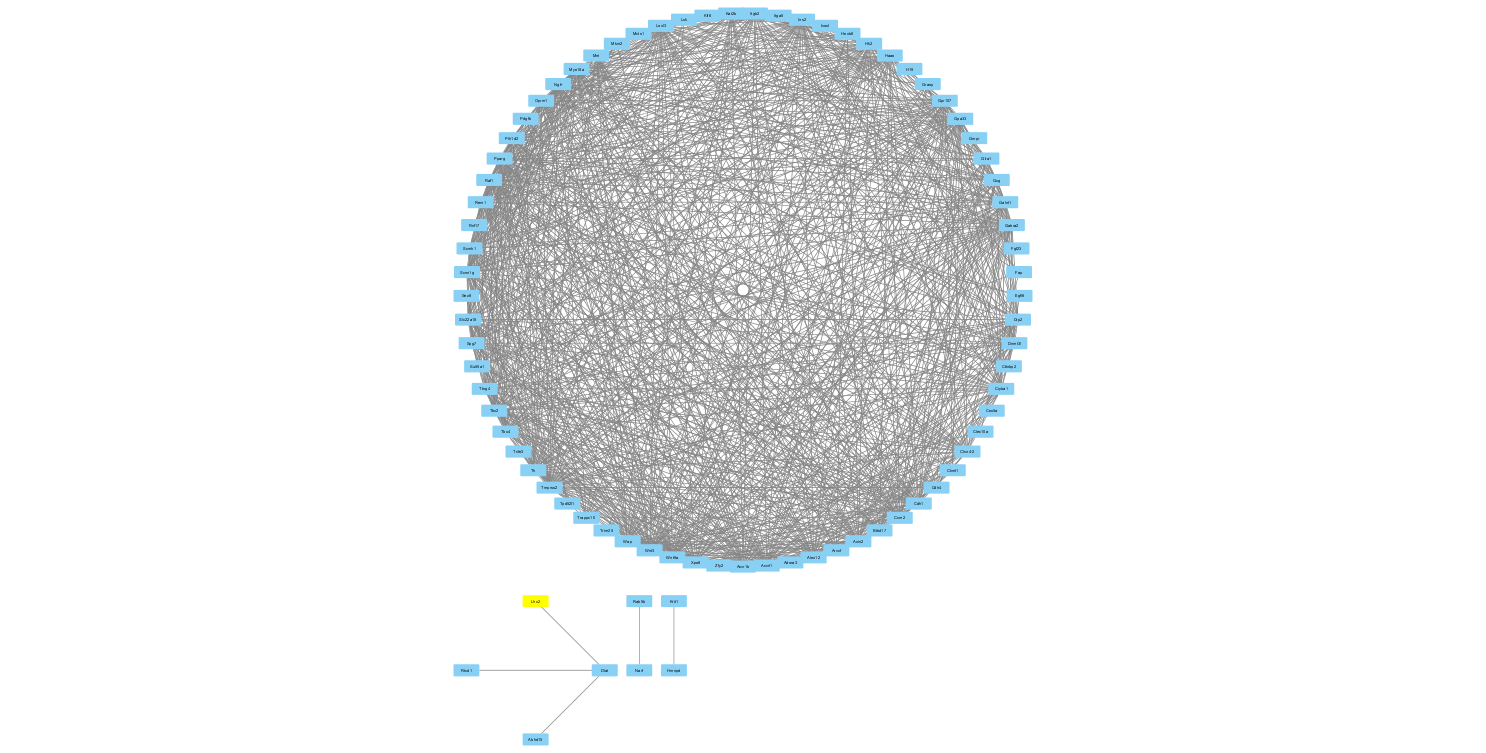
\includegraphics[width=0.9\linewidth]{img/schmitt_schowing_methylation_network_spearman}
	\caption{Methylation network with Spearman correlation}
	\label{fig:schmittschowingmethylationnetworkspearman}
\end{figure}




	% C
	\item \textbf{Discussion:}\textit{Briefly comment on the similarities and difference between the networks.
		Explain and discuss your results.}\\
	We observe that the number of correlated genes expression 
	
	
\end{enumerate}

% NEW EXERCICE
\newpage
\exercise{Blah}
\begin{enumerate}
	
	% A
	\item \textbf{Blah}\\
	
	%\lstinputlisting[label=lsdddt-1, caption={r}] {../ScriptsR/Assignment6Part2\string_schmitt\string_schowing.R}
	
	
	
\end{enumerate}

\end{document}